\documentclass[11pt,letterpaper]{article}
\usepackage[utf8]{inputenc}
\usepackage{amsmath}
\usepackage{amsfonts}
\usepackage{amssymb}
\usepackage{color}
\usepackage[margin=1in]{geometry}
\usepackage{graphicx}
\usepackage{subcaption}

\date{}
\title{\textbf{Comparison of Clustering Algorithm Performance}}
\author{Matt Bailey, Neeraj Rajesh, John Roush, Matthew Sinda \\
		\\
		Department of Computer Science \\
		Central Michigan University \\
		Mount Pleasant, Michigan  48859 \\
		\{baile5mj, rajes1n, roush2j, sinda1m\}@cmich.edu}
\begin{document}
\maketitle
\begin{abstract}
This paper examines the need for understanding the performance of clustering algorithms, details some different categories of algorithms, and then explores the current state of clustering performance analysis.  The paper then discusses an implementation for analyzing clustering performance and then details the results of running such an implementation.  Finally, the paper gives an overview of the results of running the implementation and concludes that clustering algorithm performance is highly dependent on the data set which the algorithm is clustering.
\end{abstract}

\section{Introduction}
The need to efficiently analysis and process big data is becoming more important.  2007 saw users storing 295 exabytes of digital data \cite{Hilbert}, and by 2013 the number had grown to 1,200 exabytes \cite{Lehikoinen}.  In 2013 alone, computer users stored over 13 exabytes of \textit{new} data \cite{Jagadish}, which averages over 35 petabytes per day.  When data is generated at those rates, it presents challenges, not only in the logistics of storing the data, but also in terms of how to process the data.

Data mining, the process of extracting new knowledge from data, helps solve the problem of how to analyze this wealth of data that is growing on a minute-by-minute basis.  Data mining results from a natural evolution of data storage and analysis, and it comprises a combination of statistical and technological methods for learning about data and then making predictions based on what was learned \cite{Han}.  However, simply choosing a data mining algorithm and applying it to some data set is insufficient; the sheer size of the data being analyzed means we must also consider the performance of the algorithm itself.  Consider, for example, an algorithm that runs in $O(c^n)$ time and that is used to process one million records.  This algorithm would be useless because it could never process all the records within a reasonable amount of time.  Therefore, it would be helpful to know how well some of the common data mining algorithms perform, particularly compared to one another.  To that end, we explore some common clustering algorithms, analyze their performance, both in terms of CPU and memory usage, and then look at how accurate their results are.

\section{Clustering Algorithms}
Clustering involves grouping data objects into groups, or ``clusters,'' where each data object is similar to all other objects in the cluster based on some similarity metric (usually a distance measure) \cite{Han}.  Clustering algorithms are widely used in data mining because they automatically partition data sets based on a similarity metric and can pretty easily determine which data objects are related \cite{Han}.  We chose three types of clustering algorithms to implement and analyze:  distance-based, density-based, and probabilistic.

\subsection{Distance-Based Algorithms}
Distance-based algorithms cluster data based on similarity measured by some distance metric.  We looked at two types of distance-based algorithms, $k$-means and $k$-medoids.  $k$-Means is a centroid-based partitioning algorithm that clusters data objects based on their distances to the nearest cluster center \cite{Han}.  It is an iterative process whereby data objects are assigned to clusters, the cluster centers are recomputed based on the mean of all objects in the cluster, and then the process is repeated until the cluster centers no longer change.  $k$-Means, however, is sensitive to outlier objects since outliers distort the mean values of the clusters \cite{Han}.  $k$-Medoids attempts to circumvent this problem by choosing a representative data object for each cluster.  Instead of calculating the mean of all the data object values, actual data objects are chosen such that they most accurately represent all of the data objects in their respective clusters.  The run time for the $k$-Means algorithm is O($n$)\cite{Lloyd} while the run time for k-medoids is O($n^{2}$)\cite{Kaufman}.

\subsection{Density-Based Algorithms}
Distance-based algorithms build clusters based on some distance from a cluster center, which logically produces clusters that are circular or spherical.  However, data objects do not always tend to congregate around centroids.  Density-based algorithms, on the other hand, can work around this limitation by producing clusters of arbitrary (i.e. non-spherical) shape \cite{Han}.  Instead of assigning a data object to the nearest cluster based on its distance from the cluster center, density-based algorithms consider a data object to be either part of a neighborhood (cluster) or noise, depending on surrounding objects.  To determine whether a data object resides in a cluster or not, the algorithm looks at either nearness of surrounding objects or uses a density function and noise threshold \cite{Han}.  This algorithm has a run time of O($n log n$) if an efficient lookup table is implemented\cite{Ester96}.

\subsection{Probabilistic Model-Based Algorithms}
Probabilistic model-based clustering algorithms assign data points to cluster based on a degree of membership.  That is, each data point belongs to its own cluster to some degree, but also belongs to the other clusters to lesser degrees \cite{Han}.  Probabilistic model-based algorithms determine the probability with which each data object belongs to each cluster (the degree of membership), and then assigns the point to the cluster to which it most likely belongs \cite{Han}.  This algorithm has a run time of O($n$) but is heavily influenced by the number of tuples, attributes and the number of clusters the algorithm needs to find \cite{Dempster77}.

\section{Related Works}
Comparing clustering algorithm performance in and of itself does not appear to be a widely studied area, so prior works are relatively sparse.  Instead, literature tends to focus on one of two areas:  how a newly-developed algorithm compares to an existing algorithm whose problems it was intended to solve or a survey of clustering algorithms which give a general overview of the different types.

\cite{Ester96} discusses both $k$-means and $k$-medoids, but the authors only compare their then-new DBSCAN algorithm with CLARANS, a specific $k$-medoids implementation.  For the most part, they compare DBSCAN to other clustering techniques in terms of how DBSCAN overcomes the weaknesses of other types of algorithms.  For example, the authors state that partitioning algorithms such as $k$-means and $k$-medoids can only produce convex clusters, but then show that DBSCAN is capable of producing clusters of any shape \cite{Ester96}.  Finally, \cite{Ester96} evaluates the performance of DBSCAN, but only as compared to CLARANS, not as part of a larger evaluation of clustering algorithms in general.

$k$-means was first proposed by in \cite{Lloyd}; $k$-medoids was first proposed by \cite{Kaufman}; and $c$-means, or the EM algorithm was first proposed by \cite{Dempster77}.  \cite{Nock06} evaluates and compares weighted versions four clustering algorithms:  $k$-means, fuzzy $c$-means, Gaussian EM, and harmonic means.  They first developed highly-mathematical evaluations, then devised a set of experiments that would test their versions of the algorithms in comparison with one another \cite{Nock06}.  Similar to \cite{Ester96}, the purpose of \cite{Nock06}'s experiments was not to provide a general comparison of clustering algorithms, but to test the weighted versions they developed.

\cite{Jain99} provides a general---but broad and comprehensive---overview of clustering techniques.  The authors describe the different classes of clustering algorithms, such as hierarchical, partitional, and fuzzy, and then give high-level overviews of many of the different algorithms in each class.  However, \cite{Jain99} limits its discussion of performance to generalities only, observing in one instance, for example, that artificial neural networks perform better than $k$-means and fuzzy $c$-means \cite{Jain99}.  However, they do not give specific examples of performance comparisons, nor do they devise an experiment to test the differences.

\section{Methodology}
We are interested in determining how each of our clustering algorithms performed in relation to one another, and how their performance varied with input size.  We opted to implement each algorithm from scratch in Java, along with a test framework which would generate arbitrarily sized data sets.  We look at three independent variables for performance: the number of tuples (data points), the number of attributes (dimensions), and the number of clusters.  Unless otherwise specified, all asymptotic complexity figures given in the paper refer to the number of \emph{tuples} only.

We measured runtime and memory consumption using the introspection tools of the Java Virtual Machine. In addition, we (separately) test a wide range of input sizes and configurations to gauge the accuracy of the algorithms with several different cluster quality metrics.

\subsection{Data Generation}
There are myriad sources for data sets which could be clustered, but the exact content of the data itself is not important when measuring performance.  It is, however, important to guarantee that the data does not contain hidden biases and that it covers a broad range of possible inputs.  It is also helpful to know the ``true'' clusters a priori, for the purposes of measuring each algorithms accuracy.

The core of our generator is the abstract \verb+DataGenerator.Generator+ interface (henceforth just 
\verb+Generator+).  Each \emph{class} that implements \verb+Generator+ represents an abstract cluster shape and density profile.
Our generator suite includes uniform and gaussian spheres (good for semi-randomly scattered clusters) and uniform boxes (good for building hand-crafted data sets to test edge cases).  Each \emph{instance} of these classes represents a single cluster, with an instance-specific size and center position and density multiplier.

To actually generate a data set, we take a list of clusters (i.e. generator instances) and feed in the number of dimensions, the number of tuples, and a pseudo-random seed value.  The result is a set of tuples randomly distributed amongst the clusters according to their volumes and density multipliers, and randomly positioned within their assigned cluster according to its shape and density profile.

The generated data is stored in a simple data structure, \verb+DataSet+, and passed in this form as input to our four clustering algorithms.  The ``true'' clustering of the generated data - a mapping from each tuple to its original cluster generator - is also kept for reference purposes.

A scaled-down example of generated data is shown in Figure \ref{fig:exmaplegen}.  In this case we use four normal (gaussian) circle generators with semi-random center positions against a low-density background of white noise, with a total of 1000 tuples.  During actual testing, our data sets could have dozens of clusters, span up to 50 dimensions, and contain tens of thousands of tuples.

\begin{figure}
	\centering
	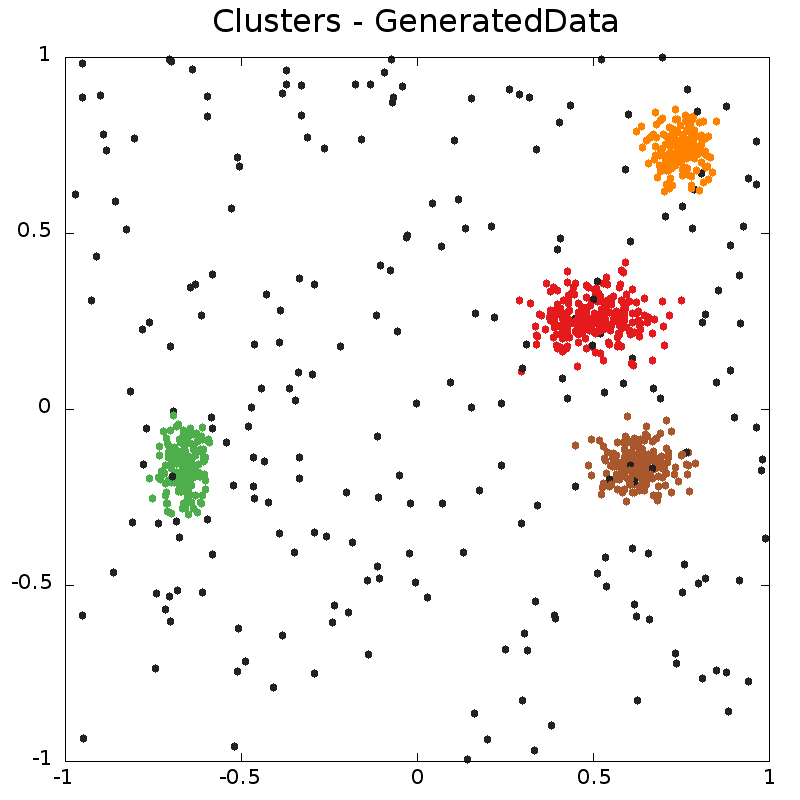
\includegraphics[width=0.8\textwidth]{{{../results-usable-clus/testdata.truth}}}
\caption{An example of generated data.}
\label{fig:exmaplegen}
\end{figure}

\subsection{Quality Metrics}
A common metric for measuring the quality of a potential clustering is the \textbf{Silhouette Coefficient}.  
Informally speaking, this combines the concepts of ``compactness'' (the average dissimilarity of objects within the same
cluster) and ``separation'' (the average dissimilarity of objects with the nearest foreign cluster).
The larger the silhouette coefficient, the better the clustering is (at least for naturally compact, convex clusters).
The silhouette for a whole clustering is the average of the coefficient of each individual data tuple:

	\[ Sl = \sum_i^N \frac{\text{sep}_i - \text{cmp}_i}{\text{max}(\text{sep}_i, \text{cmp}_i)} \]

Since the ground truth clusterings are available to us for our test data, we can also use them to directly
 evaluate cluster quality.  We use the measures \textbf{Precision} and \textbf{Recall}.  
Precision ($Pr$) is the fraction of tuples in a cluster that truly belong together, averaged over all clusters.  
Recall ($Rc$) is the fraction of objects belonging together (in the same 
``true'' cluster) that are clustered together, averaged over all ``true'' 
clusters.  The larger both metrics are (up to a maximum of 1.0), the better the clustering corresponds
with the ``ground truth''.

\subsection{Clustering Algorithm Implementations}
Each of the four clustering algorithms was implemented on top of an abstract Java class, \verb+Clustering+.
This class documents the interface that each algorithm must provide.  Simply put, each clustering algorithm
was given a \verb+DataSet+ and, if necessary, the number of ``true'' clusters as input.  The output was a mapping
from data tuples to clusters.

There are many different algorithms for distance-based, density-based, and probabilistic model-based clustering.  We chose to implement four specific clustering algorithms:  $k$-means and PAM (distance-based), DBSCAN (density-based), and EM (probabilistic-based).

\subsubsection{\textit{k}-Means} 
The $k$-means implementation is fairly straightforward.  It takes initial cluster centers, iterates through each tuple in the data set and assigns it to a cluster based on the closest center, recalculates the centers according to the mean values for each attribute in the tuples, and then starts the process over.  This process continues until there are no more changes in the cluster assignments.

The $k$-means algorithm could be considered one of the simplest algorithms in terms of understanding and implementation.  There are no nested \verb+for+ loops, so the algorithms runs in $O(n)$ time.  The only potential problem is that $k$-means assigns every tuple to a cluster, so it is sensitive to noise.  In addition, extreme outliers have great potential to skew the clusters.

\subsubsection{PAM}
Partitioning Around Medoids (PAM) is an algorithm that performs $k$-medoids clustering.  PAM uses representative objects from the data set.  That is, the algorithm tries to find one object per cluster that most accurately represents all of the object in the cluster.  PAM requires ``seed'' objects---initial starting tuples from the data set---which are arbitrarily chosen to represent initial clusters.  It then begins an iterative process whereby it replaces representative objects with other objects until the best possible clusters are produced, which is tested by calculating the absolute error.

PAM uses a greedy method by choosing the object with the lowest cost as determined by the average dissimilarity between the object and its cluster representative.  Despite using a greedy method, PAM is an inherently inefficient algorithm as it ultimately checks each object against all other objects in an iterative manner; our implementation uses nested \verb+for+ loops to mimic this behavior, which causes the algorithm to run in $O(n^{2})$ time.

\subsubsection{DBSCAN} 
Density-Based Spatial Clustering of Applications with Noise (DBSCAN) is a density-based clustering algorithm. DBSCAN uses two user-specified parameters, epsilon ($\epsilon$) and minimum points ($MinPts$), to find regions of dense ``neighborhoods'' of data objects, which are then considered clusters.  Density is a function of the radius of the neighborhood, specified by $\epsilon$, and a neighborhood is defined by $MinPts$.  That is, for each data object in the data set, DBSCAN looks at how many other objects are within a radius of $\epsilon$, and if that value is greater than or equal to $MinPts$, then the object is considered a core object.  From there, DBSCAN finds small dense regions by connecting core objects with respect to $\epsilon$ and $MinPts$, and finally it builds large dense regions by connecting objects within a radius of $\epsilon$ of already-connected objects.

The biggest limiting factor with our DBSCAN implementation proved to be with regard to the the data set implementation.
The original specification of the algorithm assumes an efficient $O(lg n)$ way to locate the nearest neighbors of any given
tuple.  We chose to store the tuples in a flat array for simplicity, and we did not implement any fast lookup mechanisms.
Thus, our implementation requires $O(n)$ to find the nearest neighbors of a tuple, and the algorithm itself runs in $O(n^2)$ time.

\subsubsection{EM} 
Expectation-maximization (EM) is a technique for producing fuzzy clusters and probabilistic model-based clusters.  EM starts with randomly-selected objects as potential centers and then iteratively works in two steps:  the expectation step and the maximization step.  The expectation step iterates through each data object, calculates the distance to each of the potential centers, and then calculates a partition matrix containing values that indicate to what degree each object belongs to a cluster centered at each of the potential centers.  The partition matrix, containing membership weights, is then normalized so the sum of degrees for each object is 1.  Next, the maximization step uses the partition matrix to recalculate the centroids, by calculating an optimal center and then finding the data object closest to that optimal center.  The process repeats until the clusters stop changing or until the change is below some predefined threshold.

EM runs until there are no more changes.  Despite running in $O(n)$ time, there is potential for the algorithm not to converge, but to end up with increasingly smaller changes, which requires a threshold to determine when to stop running the algorithm.

\section{Results}
We looked at the results of the clustering algorithms both in terms of how accurately each algorithm calculated clusters compared to what we were expecting (i.e. the ``ground truth'') and in terms of performance (both run time and memory usage).  Section \ref{ssec:clusters} gives the results of the generated clusters on varying types of data sets, and Section \ref{ssec:performance} gives the absolute performance results.

\subsection{Clustering Results}\label{ssec:clusters}
\begin{figure}
	\centering
	\begin{subfigure}[b]{0.3\textwidth}
	\centering
	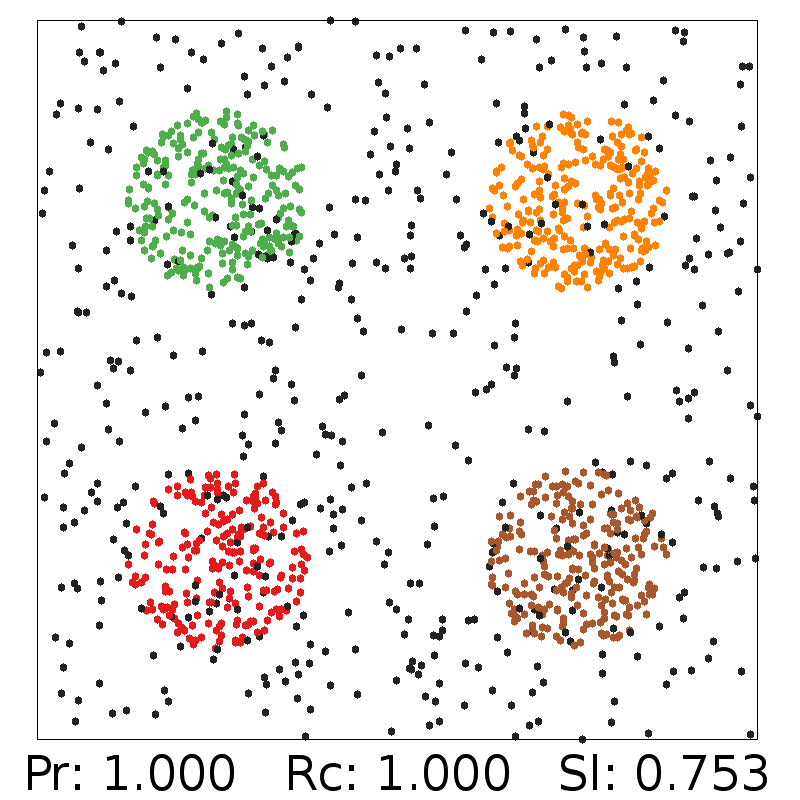
\includegraphics[scale=0.2]{{{../results-usable-clus/basicnoise.truth}}}
	\caption{Ground truth}
	\label{fig:expected-basic}
	\end{subfigure}%
	\begin{subfigure}[b]{0.3\textwidth}
	\centering
	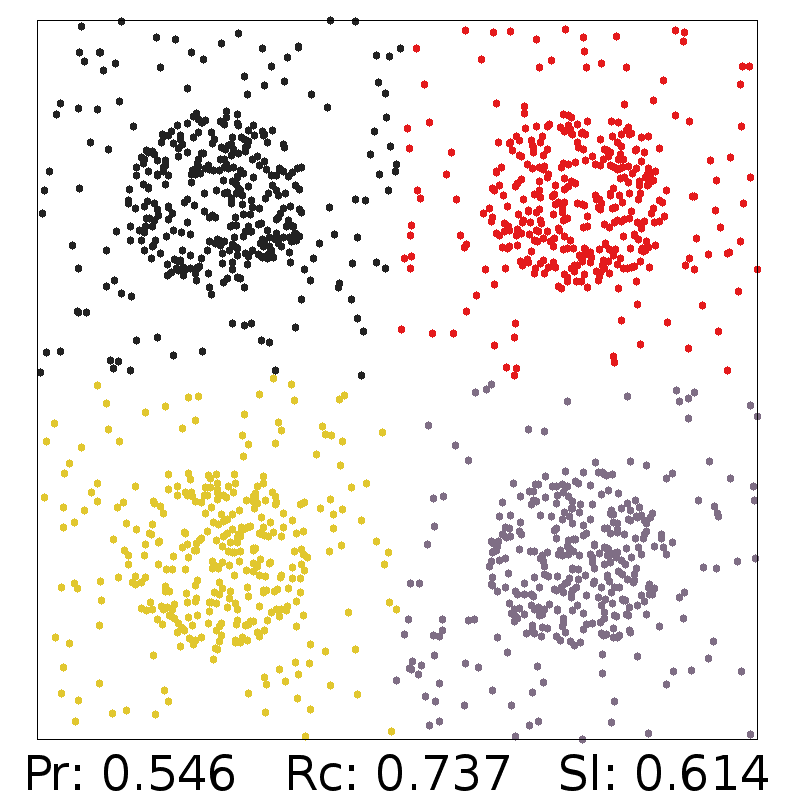
\includegraphics[scale=0.2]{{{../results-usable-clus/basicnoise.kmeans}}}
	\caption{$k$-means}
	\label{fig:kmeans-basic}
	\end{subfigure}%
	\begin{subfigure}[b]{0.3\textwidth}
	\centering
	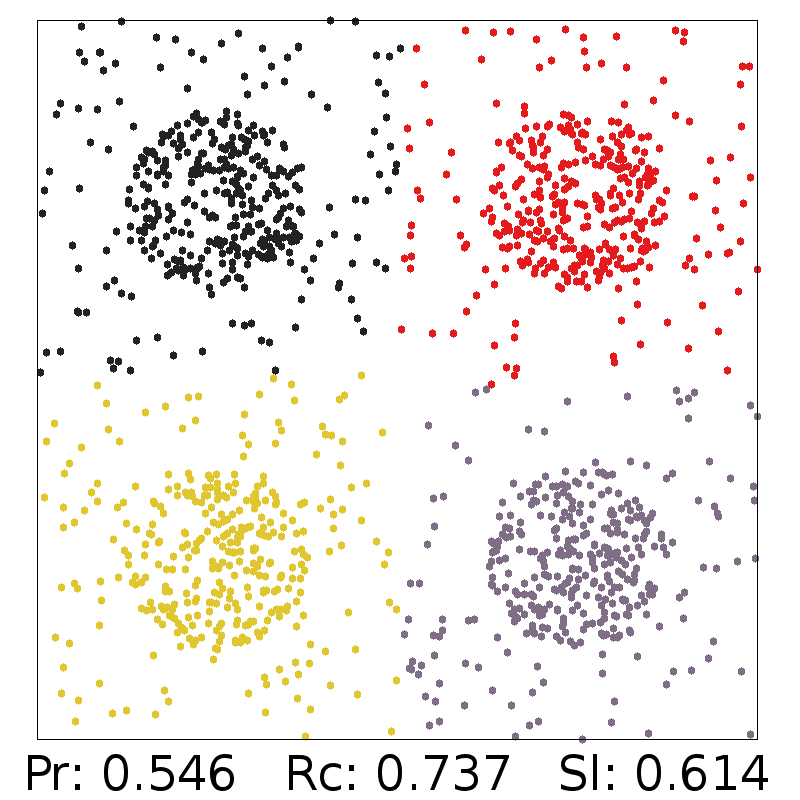
\includegraphics[scale=0.2]{{{../results-usable-clus/basicnoise.kmedoids}}}
	\caption{PAM}
	\label{fig:kmedoids-basic}
	\end{subfigure}
	\begin{subfigure}[b]{0.3\textwidth}
	\centering
	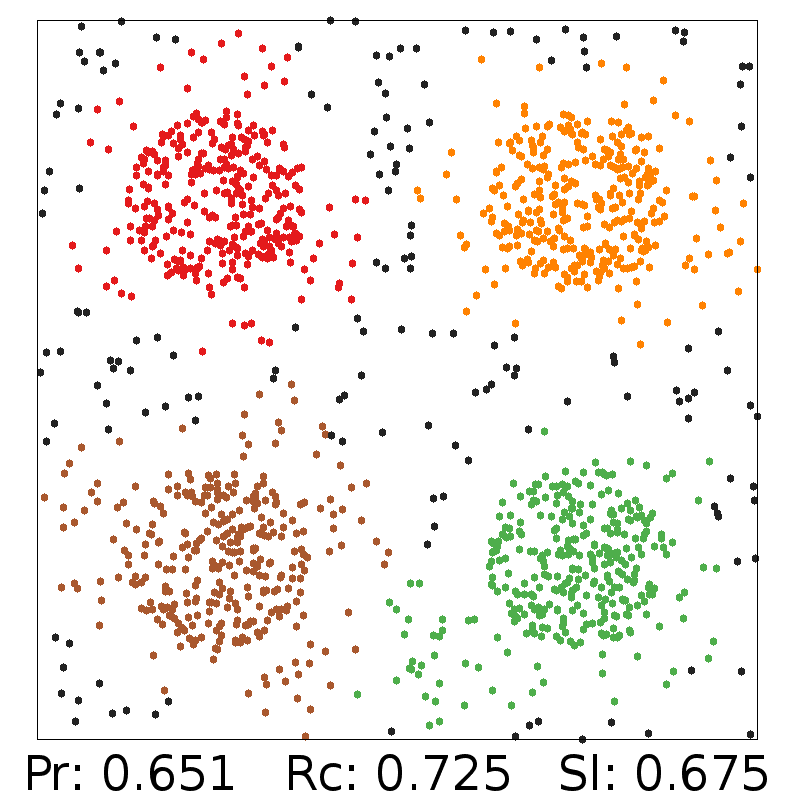
\includegraphics[scale=0.2]{{{../results-usable-clus/basicnoise.dbscan}}}
	\caption{DBSCAN}
	\label{fig:dbscan-basic}
	\end{subfigure}%
	\begin{subfigure}[b]{0.3\textwidth}
	\centering
	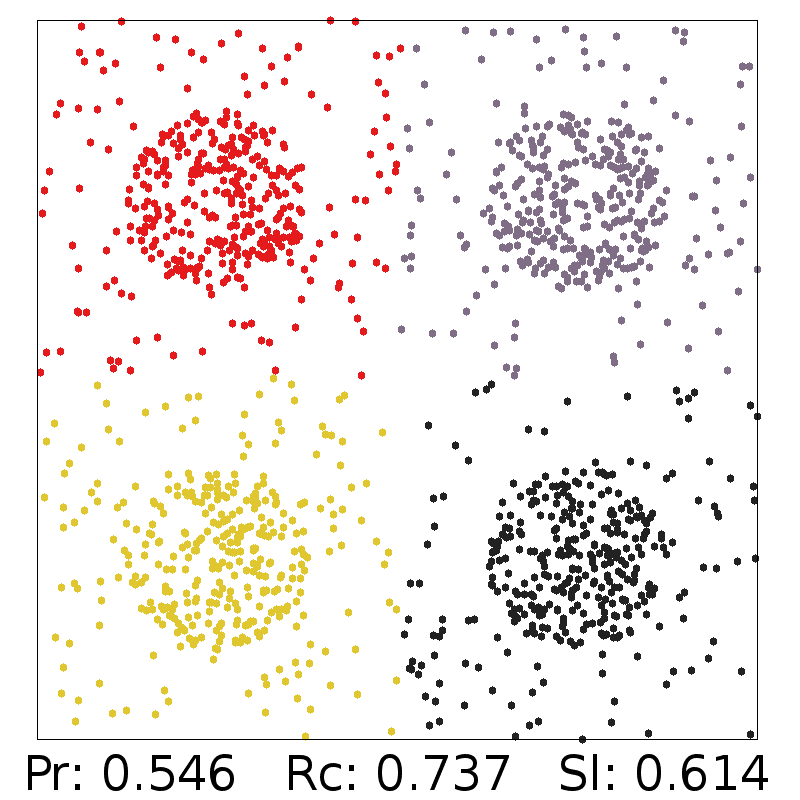
\includegraphics[scale=0.2]{{{../results-usable-clus/basicnoise.cmeans}}}
	\caption{EM}
	\label{fig:cmeans-basic}
	\end{subfigure}
\caption{Clustering results on spherical clusters with random noise.}
\label{fig:basic}
\end{figure}

Figure \ref{fig:basic} illustrates the results of clustering a basic data set with random noise points.  As we can see in Figure \ref{fig:dbscan-basic}, DBSCAN produced the most precise results, successfully distinguishing noise from cluster points, and coming closest to matching the ground truth (Figure \ref{fig:expected-basic}).  On the other hand, $k$-means, PAM, and EM all produced relatively similar results, clustering all points without regard to noise.

\begin{figure}
	\centering
	\begin{subfigure}[b]{0.3\textwidth}
	\centering
	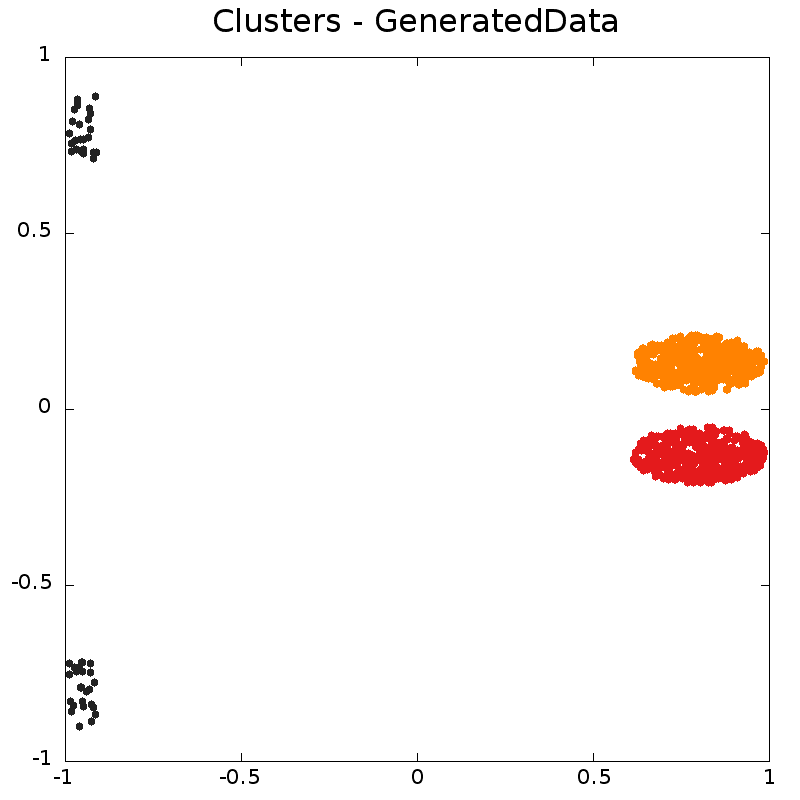
\includegraphics[scale=0.2]{{{../results-usable-clus/outliers.truth}}}
	\caption{Ground truth}
	\label{fig:expected-outliers}
	\end{subfigure}%	
	\begin{subfigure}[b]{0.3\textwidth}
	\centering
	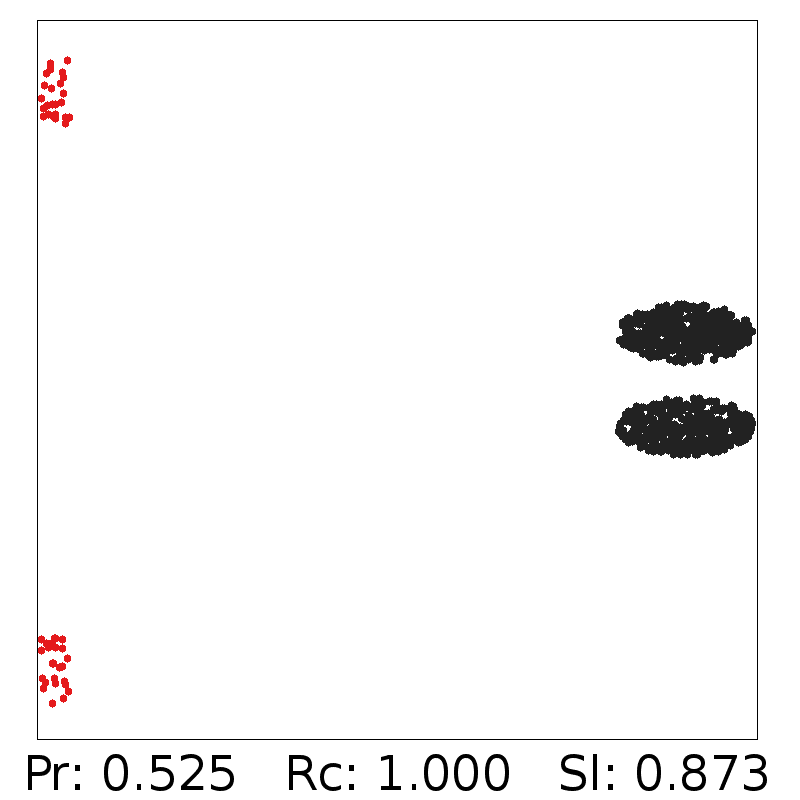
\includegraphics[scale=0.2]{{{../results-usable-clus/outliers.kmeans}}}
	\caption{$k$-means}
	\label{fig:kmeans-outliers}
	\end{subfigure}%
	\begin{subfigure}[b]{0.3\textwidth}
	\centering
	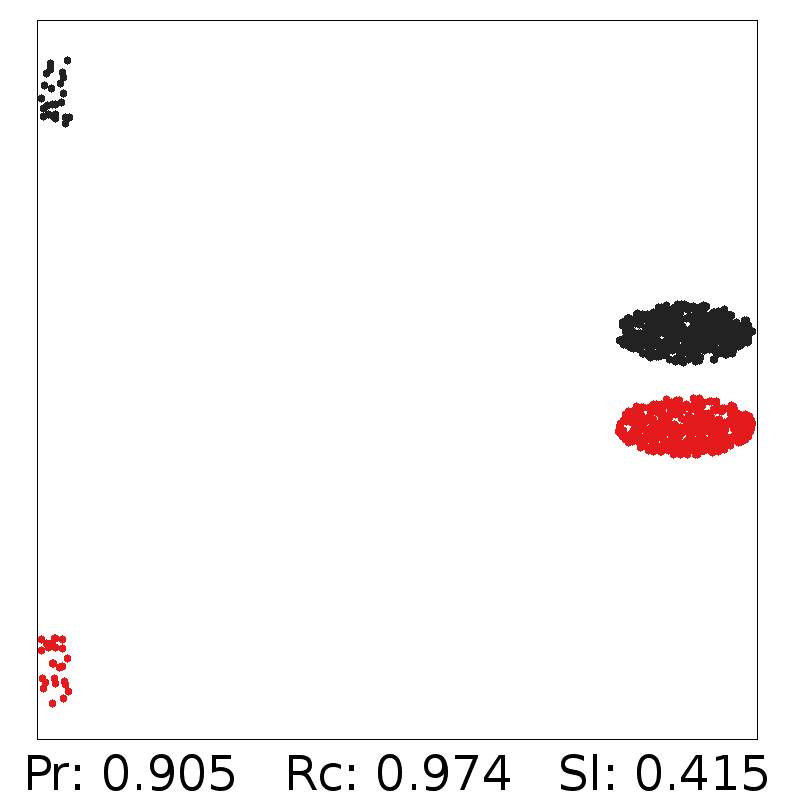
\includegraphics[scale=0.2]{{{../results-usable-clus/outliers.kmedoids}}}
	\caption{PAM}
	\label{fig:kmedoids-outliers}
	\end{subfigure}
	
	\begin{subfigure}[b]{0.3\textwidth}
	\centering
	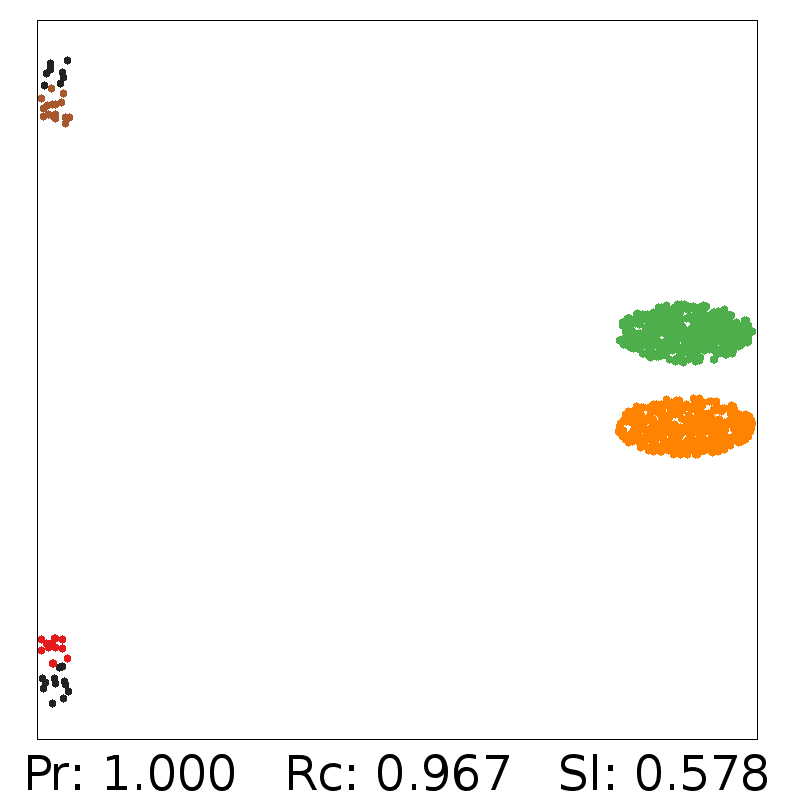
\includegraphics[scale=0.2]{{{../results-usable-clus/outliers.dbscan}}}
	\caption{DBSCAN}
	\label{fig:dbscan-outliers}
	\end{subfigure}%
	\begin{subfigure}[b]{0.3\textwidth}
	\centering
	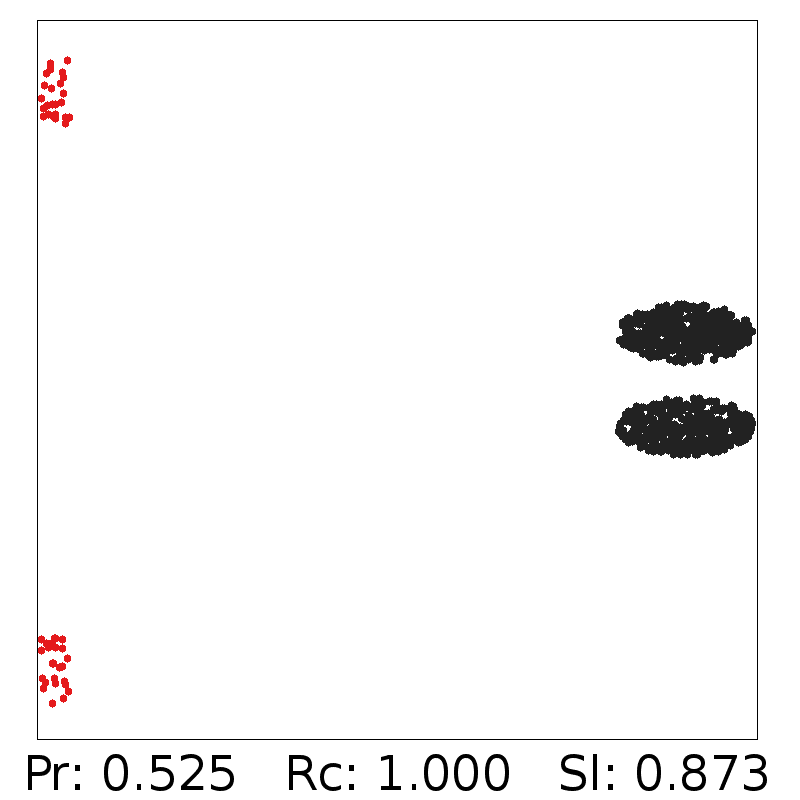
\includegraphics[scale=0.2]{{{../results-usable-clus/outliers.cmeans}}}
	\caption{EM}
	\label{fig:cmeans-outliers}
	\end{subfigure}
\caption{Clustering results on spherical clusters with extreme outliers.}
\label{fig:outliers}
\end{figure}

Figure \ref{fig:outliers} shows a data containing extreme outlying points rather than random noise.  In this instance, both DBSCAN and PAM do quite well.  $k$-means and EM mistakenly clump the two oval clusters together and put the outliers in their own cluster.  This highlights the particular weakness of these two algorithms, which both rely on geometric means and are therefore sensitive to outliers.  Notably, PAM uses median tuples and does not have this weakness.

\begin{figure}
	\centering
	\begin{subfigure}[b]{0.3\textwidth}
	\centering
	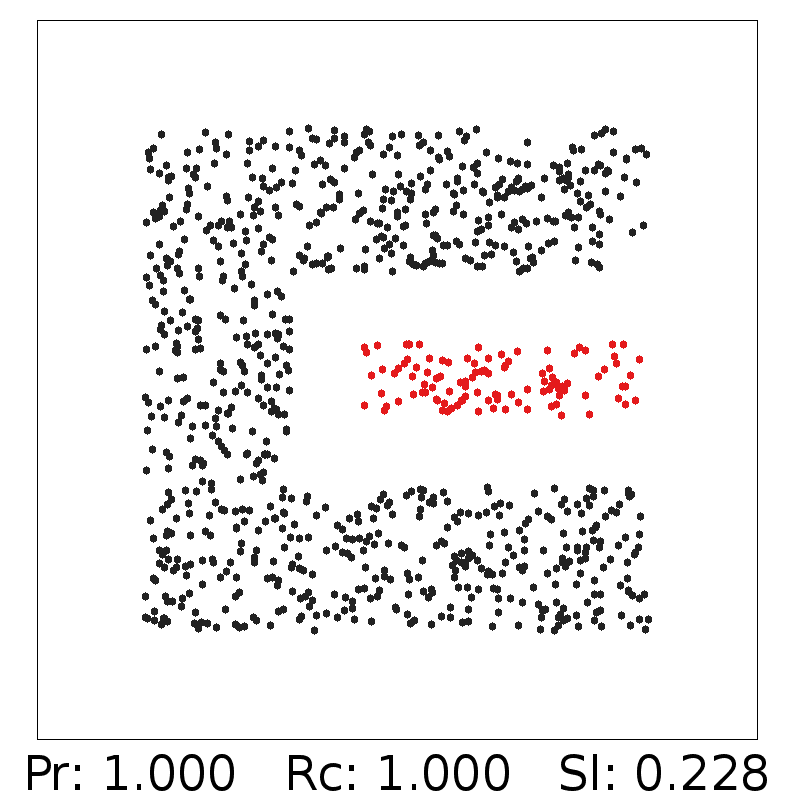
\includegraphics[scale=0.2]{{{../results-usable-clus/concave.truth}}}
	\caption{Ground truth}
	\label{fig:expected-concave}
	\end{subfigure}%	
	\begin{subfigure}[b]{0.3\textwidth}
	\centering
	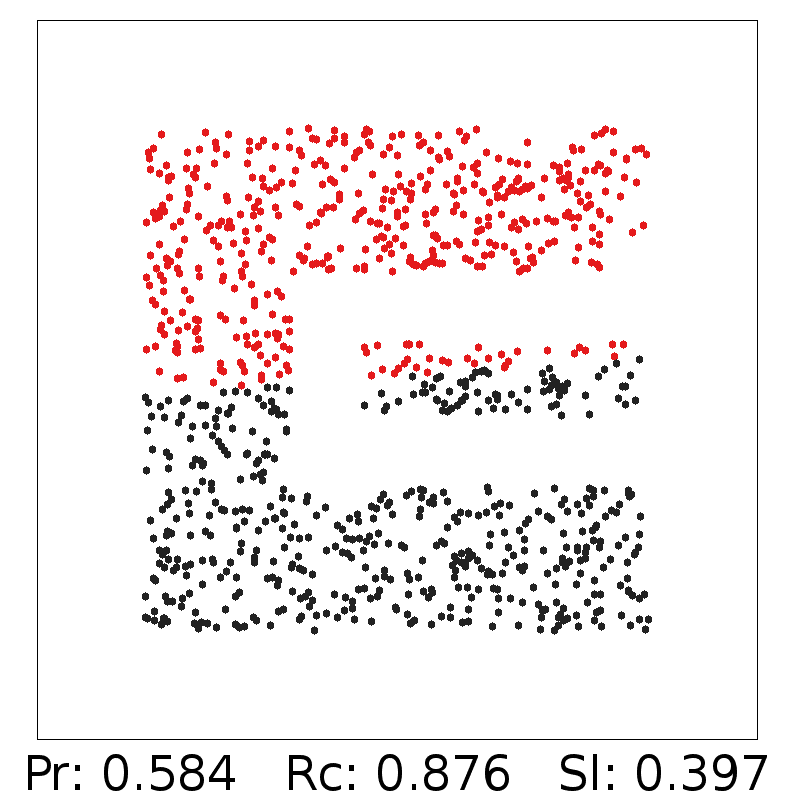
\includegraphics[scale=0.2]{{{../results-usable-clus/concave.kmeans}}}
	\caption{$k$-means}
	\label{fig:kmeans-concave}
	\end{subfigure}%
	\begin{subfigure}[b]{0.3\textwidth}
	\centering
	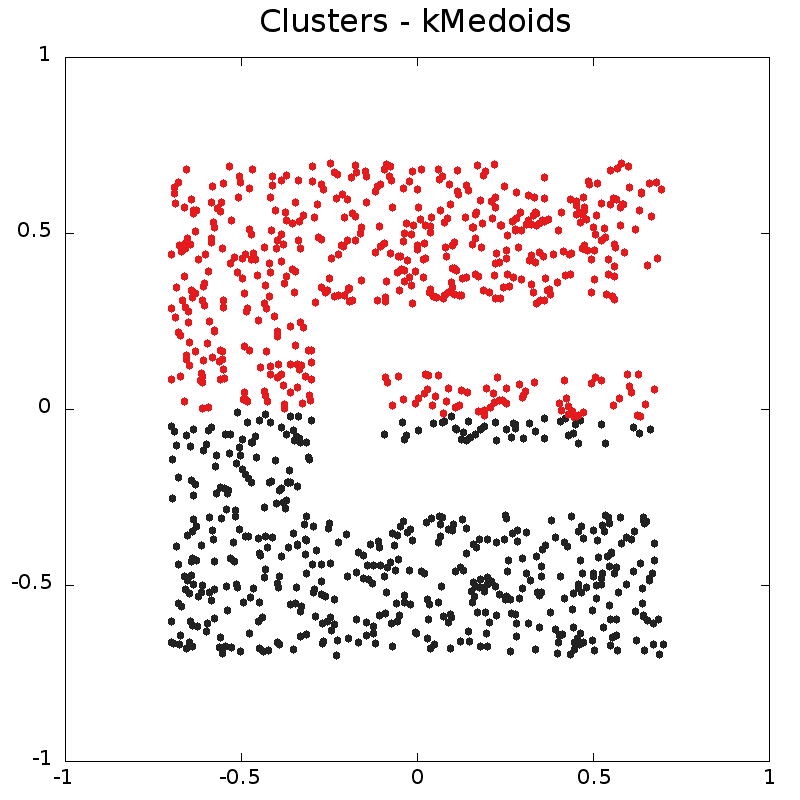
\includegraphics[scale=0.2]{{{../results-usable-clus/concave.kmedoids}}}
	\caption{PAM}
	\label{fig:kmedoids-concave}
	\end{subfigure}	
	\begin{subfigure}[b]{0.3\textwidth}
	\centering
	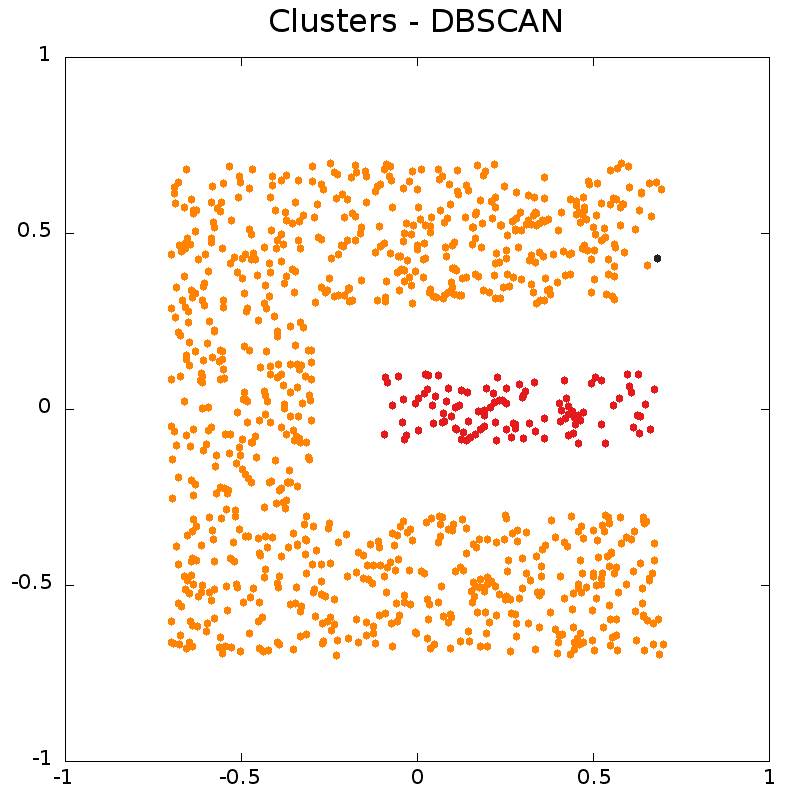
\includegraphics[scale=0.2]{{{../results-usable-clus/concave.dbscan}}}
	\caption{DBSCAN}
	\label{fig:dbscan-concave}
	\end{subfigure}%
	\begin{subfigure}[b]{0.3\textwidth}
	\centering
	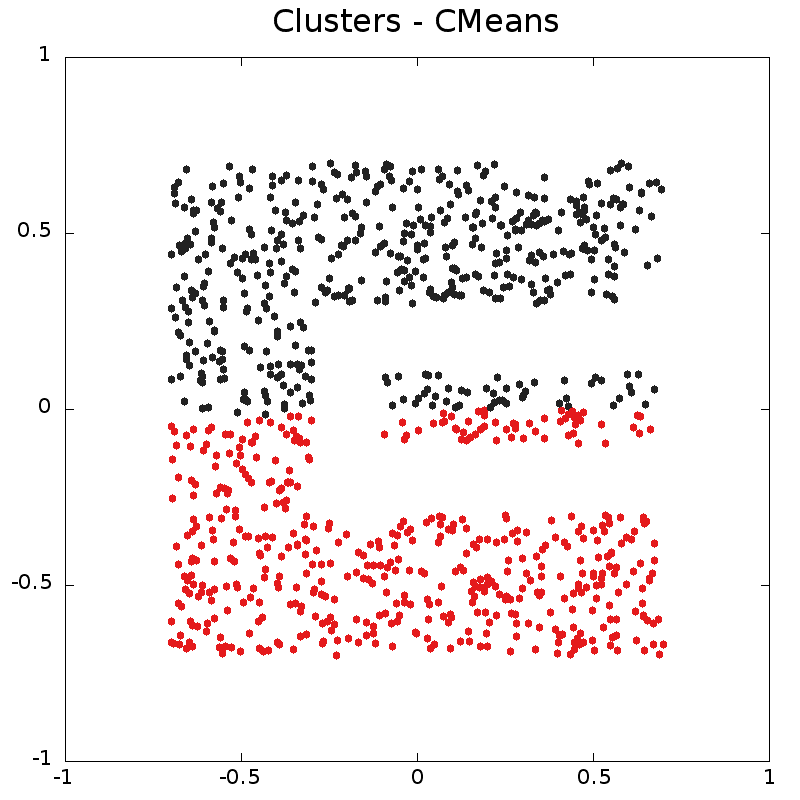
\includegraphics[scale=0.2]{{{../results-usable-clus/concave.cmeans}}}
	\caption{EM}
	\label{fig:cmeans-concave}
	\end{subfigure}
\caption{Clustering results on a concave cluster.}
\label{fig:concave}
\end{figure}

We can also see in Figure \ref{fig:concave} that DBSCAN performs the best when picking out a concave cluster.  This highlights the weakness of the other three algorithms, which all use distance to a cluster prototype and therefore are
heavily biased towards compact, convex clusters.

Overall, DBSCAN appears to be the most robust algorithm to edge cases and odd cluster shapes. Although it did not produce 100\% accurate results, it was relatively accurate, particularly with its ability to distinguish noise points from clusters points.  On the other hand, $k$-means, PAM, and EM all produced essentially similar results regardless of the data set, so we must look at their memory and CPU performance to see if there are any distinguishing characteristics.

\subsection{Performance}\label{ssec:performance} 
\begin{figure}
	\centering
	\begin{subfigure}[b]{0.45\textwidth}
	\centering
	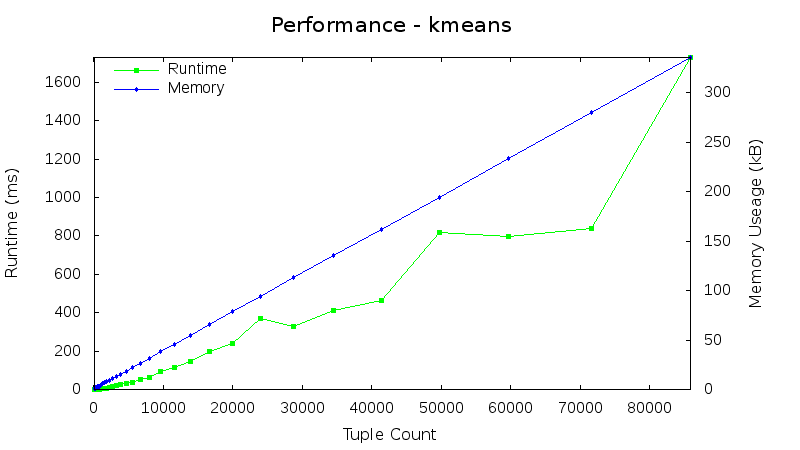
\includegraphics[scale=0.38]{{{../results-usable-perf/kmeans.tupleperf}}}
	\caption{$k$-means}
	\label{fig:kmeans-perf-tuple}
	\end{subfigure}\qquad%
	\begin{subfigure}[b]{0.45\textwidth}
	\centering
	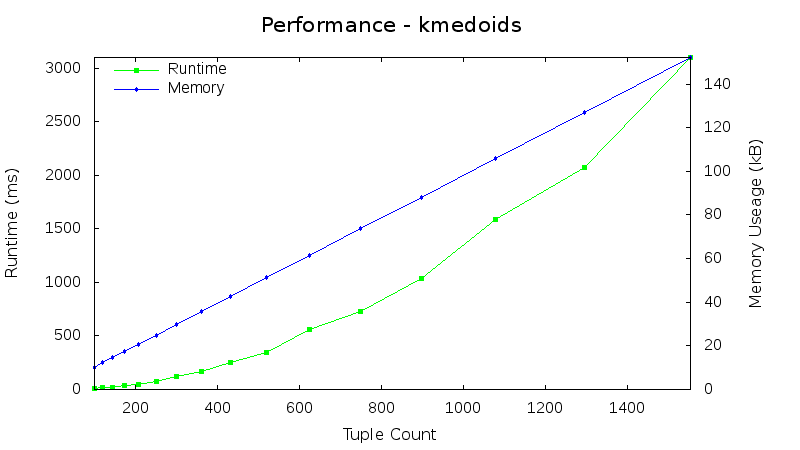
\includegraphics[scale=0.38]{{{../results-usable-perf/kmedoids.tupleperf}}}
	\caption{PAM}
	\label{fig:pam-perf-tuple}
	\end{subfigure}
	
	\begin{subfigure}[b]{0.45\textwidth}
	\centering
	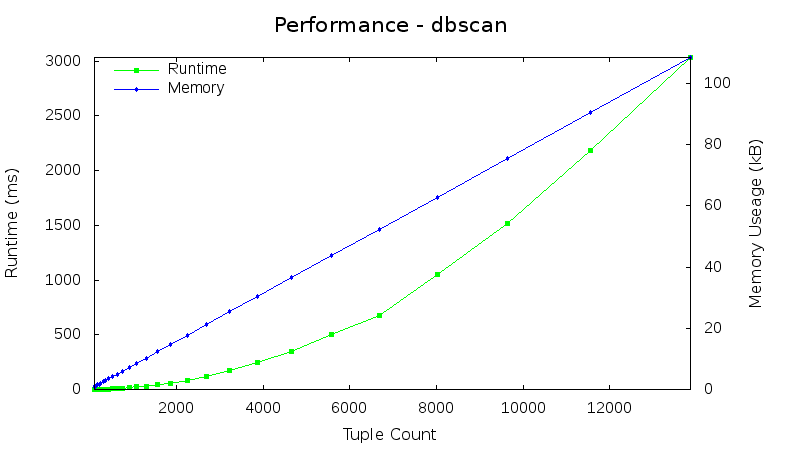
\includegraphics[scale=0.38]{{{../results-usable-perf/dbscan.tupleperf}}}
	\caption{DBSCAN}
	\label{fig:dbscan-perf-tuple}
	\end{subfigure}\qquad%
	\begin{subfigure}[b]{0.45\textwidth}
	\centering
	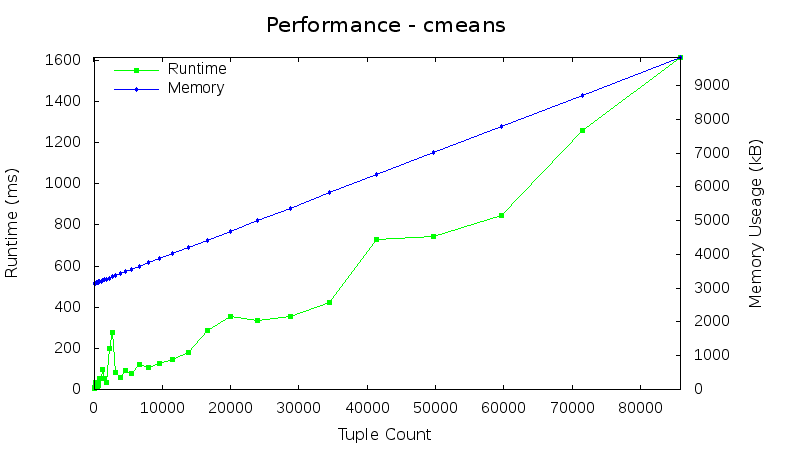
\includegraphics[scale=0.38]{{{../results-usable-perf/cmeans.tupleperf}}}
	\caption{EM}
	\label{fig:em-perf-tuple}
	\end{subfigure}
	\caption{Performance of algorithm implementations based on increasing number of tuples.}
	\label{fig:perf-tuple}
\end{figure}

Figure \ref{fig:perf-tuple} shows how our implementations performed as the number of tuples in the data set increased.  All four algorithms performed about the same in terms of memory usage:  memory consumption increased linearly as the number of tuples increased.  In terms of maximum memory usage, though, $k$-means outperformed the others by consuming no more than 40 KB of memory.  By contrast, EM was the clear loser at a maximum of 11 MB.

We can also see some difference in the algorithms in terms of time performance.  Figures \ref{fig:pam-perf-tuple} and \ref{fig:dbscan-perf-tuple} show that PAM and DBSCAN run in $O(n^2)$ time, which is consistent with our expectations.  On the other hand, the functions describing the running times for $k$-means and EM are not immediately clear, although further testing may reveal their performance trends.  Figures \ref{fig:kmeans-perf-tuple} and \ref{fig:em-perf-tuple} show that time to cluster did not steadily increase, but instead tended to have relative ups and downs with an overall upward trend.  Additionally, Figure \ref{fig:em-perf-tuple} shows a dramatic increase in run time as the data set increased from about 6,000 to 7,000 tuples, followed by a dramatic relative decrease in run time as the data set increased from about 7,000 to 8,000 tuples.

\begin{figure}
	\centering
	\begin{subfigure}[b]{0.45\textwidth}
	\centering
	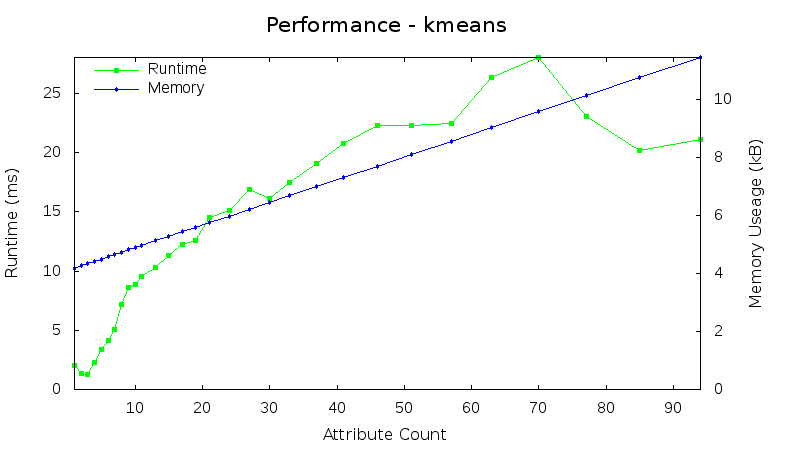
\includegraphics[scale=0.38]{{{../results-usable-perf/kmeans.attrperf}}}
	\caption{$k$-means}
	\label{fig:kmeans-perf-attribute}
	\end{subfigure}\qquad%
	\begin{subfigure}[b]{0.45\textwidth}
	\centering
	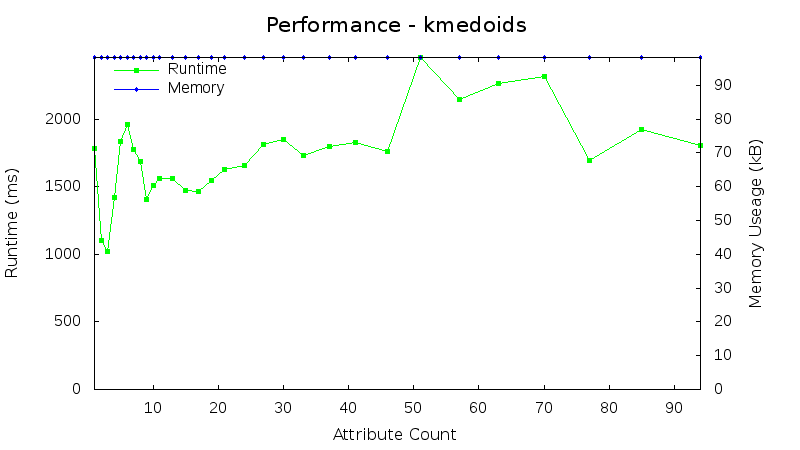
\includegraphics[scale=0.38]{{{../results-usable-perf/kmedoids.attrperf}}}
	\caption{PAM}
	\label{fig:pam-perf-attribute}
	\end{subfigure}
	
	\begin{subfigure}[b]{0.45\textwidth}
	\centering
	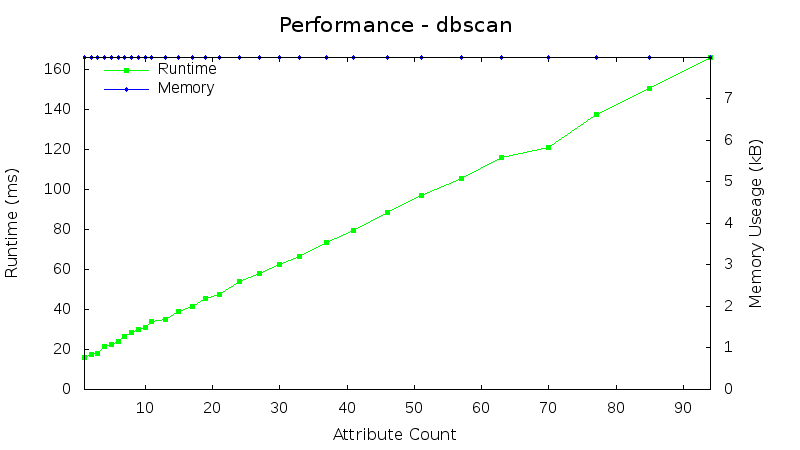
\includegraphics[scale=0.38]{{{../results-usable-perf/dbscan.attrperf}}}
	\caption{DBSCAN}
	\label{fig:dbscan-perf-attribute}
	\end{subfigure}\qquad%
	\begin{subfigure}[b]{0.45\textwidth}
	\centering
	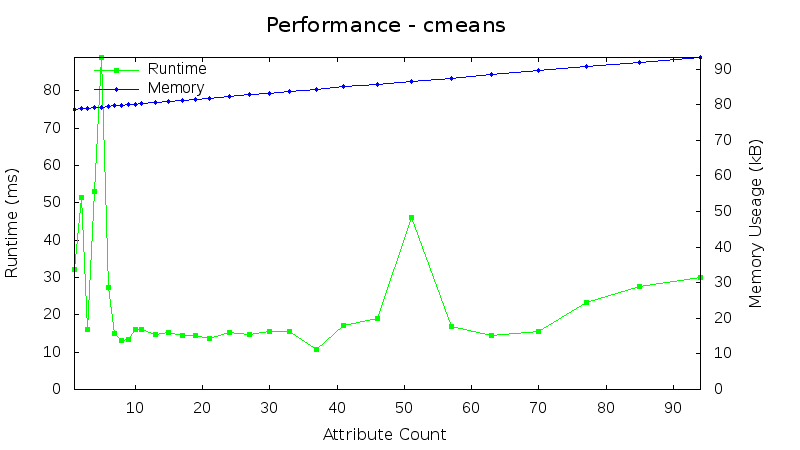
\includegraphics[scale=0.38]{{{../results-usable-perf/cmeans.attrperf}}}
	\caption{EM}
	\label{fig:em-perf-attribute}
	\end{subfigure}
	\caption{Performance of algorithm implementations based on increasing number of attributes per tuple.}
	\label{fig:perf-attribute}
\end{figure}

Assuming that Figures \ref{fig:kmeans-perf-tuple} and \ref{fig:em-perf-tuple} do indeed show linear trends, we can compare our results to the theoretical expectations.  In table \ref{tab:runTimes}, we match the asymptotic run time of our implementation against that of the original proposed algorithm.  We matched the run times for all algorithms except for DBSCAN.  This mismatch is due to our lack of an efficient spatial lookup method for this algorithm, omitted for time (and complexity!) concerns.   

\begin{table} [!h]
	\centering
	\begin{tabular}{|c|c|c|}
		\hline
		 & Implementation & Original \\ \hline
		 PAM & O($n^{2}$) & O($n^{2}$) \\ \hline
		 $k$-means & O($n$) & O($n$) \\ \hline
		 EM & O($n$) & O($n$) \\ \hline
		 DBSCAN & O($n^2$) & O($n log n$)\\ \hline
	\end{tabular}
	\caption{Comparison of Run Times} \label{tab:runTimes}
\end{table}

Figure \ref{fig:perf-attribute} illustrates that the number of attributes in each tuple had a dramatic effect on the performance of some of the algorithms.  In terms of memory usage, Figures \ref{fig:kmeans-perf-attribute}, \ref{fig:pam-perf-attribute}, and \ref{fig:em-perf-attribute} show that $k$-means, PAM, and EM were all relatively stable and that the usage for all three increased linearly as the number of attributes increased.  DBSCAN, however, exhibited ups and downs in its memory usage as shown in Figure \ref{fig:dbscan-perf-attribute}, which could potentially be a result of Java's garbage collector dynamically allocating and deallocating memory.

Figures \ref{fig:kmeans-perf-attribute}, \ref{fig:pam-perf-attribute}, and \ref{fig:dbscan-perf-attribute} show that $k$-means, PAM, and DBSCAN saw a relatively linear increase in running time as the number of attributes increased.  EM's running time, as seen in Figure \ref{fig:em-perf-attribute}, spiked near the beginning of the test, and then remained relatively constant once the number of attributes increased from about seven onward.  Overall, though, PAM appeared to be the most performant in terms of both time and memory.

\begin{figure}
	\begin{subfigure}[b]{0.45\textwidth}
	\centering
	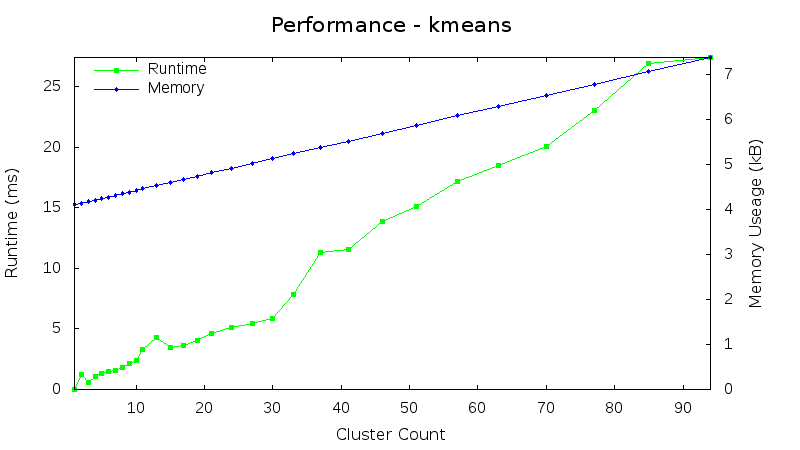
\includegraphics[scale=0.38]{{{../results-usable-perf/kmeans.clusperf}}}
	\caption{$k$-means}
	\label{fig:kmeans-perf-cluster}
	\end{subfigure}\qquad%
	\begin{subfigure}[b]{0.45\textwidth}
	\centering
	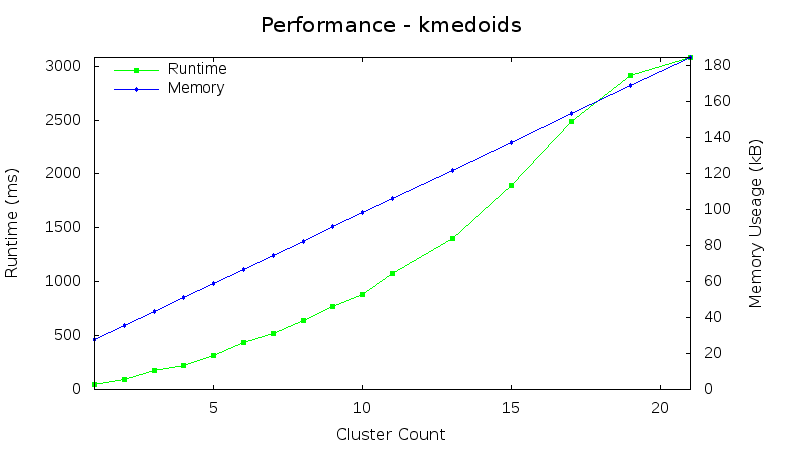
\includegraphics[scale=0.38]{{{../results-usable-perf/kmedoids.clusperf}}}
	\caption{PAM}
	\label{fig:pam-perf-cluster}
	\end{subfigure}
	
	\begin{subfigure}[b]{0.45\textwidth}
	\centering
	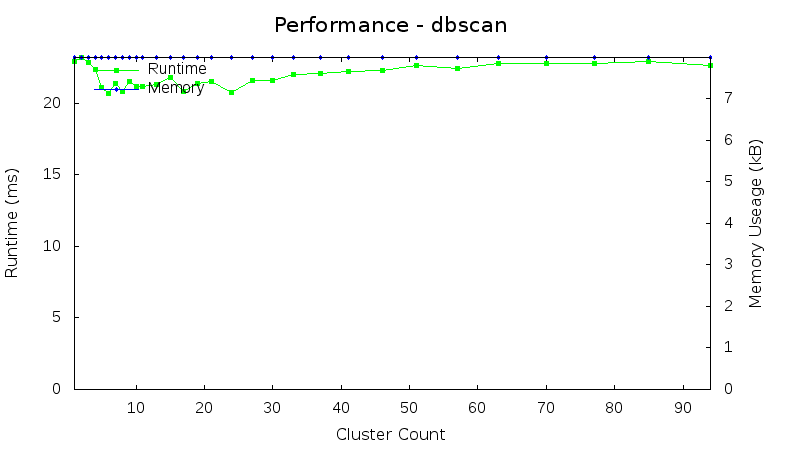
\includegraphics[scale=0.38]{{{../results-usable-perf/dbscan.clusperf}}}
	\caption{DBSCAN}
	\label{fig:dbscan-perf-cluster}
	\end{subfigure}\qquad%
	\begin{subfigure}[b]{0.45\textwidth}
	\centering
	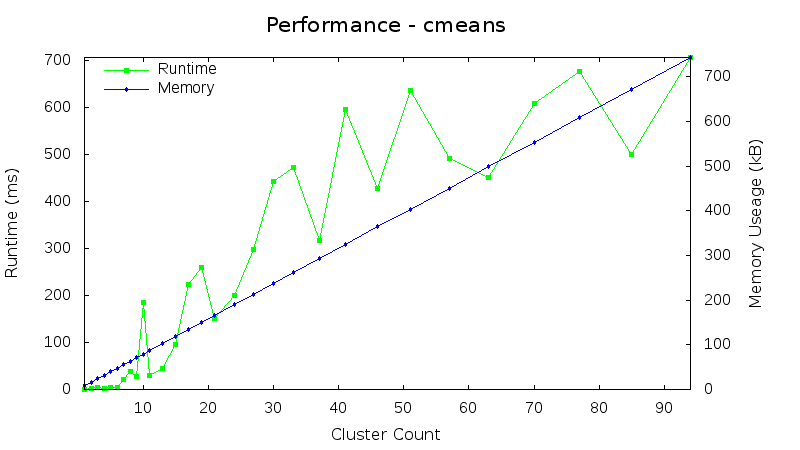
\includegraphics[scale=0.38]{{{../results-usable-perf/cmeans.clusperf}}}
	\caption{EM}
	\label{fig:em-perf-cluster}
	\end{subfigure}
	\caption{Performance of algorithm implementations based on increasing number clusters to find.}
	\label{fig:perf-cluster}
\end{figure}

Figure \ref{fig:perf-cluster} shows performance as the cluster count increases.  Figures \ref{fig:kmeans-perf-cluster} and \ref{fig:pam-perf-cluster} show that both $k$-means and PAM saw a relatively linear increase in both processing time and memory usage.  EM also saw a linear increase in memory usage as seen if Figure \ref{fig:em-perf-cluster}.  On the other hand, DBSCAN's memory performance was much the same as when the number of attributes were increasing.  Again, this could be because of dynamic memory (de)allocation during the program's run.

In terms of time performance, both DBSCAN and EM were relatively unstable as Figures \ref{fig:dbscan-perf-cluster} and \ref{fig:em-perf-cluster} show.  However, DBSCAN's running time did not exhibit quite as much relative variation as EM's did.  Overall, $k$-means and PAM appear to be tied for best performance, with a slight edge going to $k$-means.

\section{Conclusion}
Ultimately, no one algorithm stands out as being the best.  Instead, each algorithm seems best-suited for different applications.  Going in to the project, we were aware that $k$-means, $k$-medoids, and fuzzy $c$-means were all sensitive to outliers, which is apparent in the cluster plots.  However, we did not know that each algorithm (including DBSCAN) would be better suited to different types of data sets than the others.  For example, DBSCAN tended to perform worse than the others, but was most accurate at creating clusters that match those of the original data set.  In the end, we can conclude that clustering analysis should involve clustering the data using more than one algorithm and then choosing the one that produces the most accurate results.

\bibliographystyle{plain}
\bibliography{sources}

\newpage
\appendix
\section{Appendix A - Additional Plots}

\begin{figure}[h]
	\centering
	\begin{subfigure}[b]{0.3\textwidth}
	\centering
	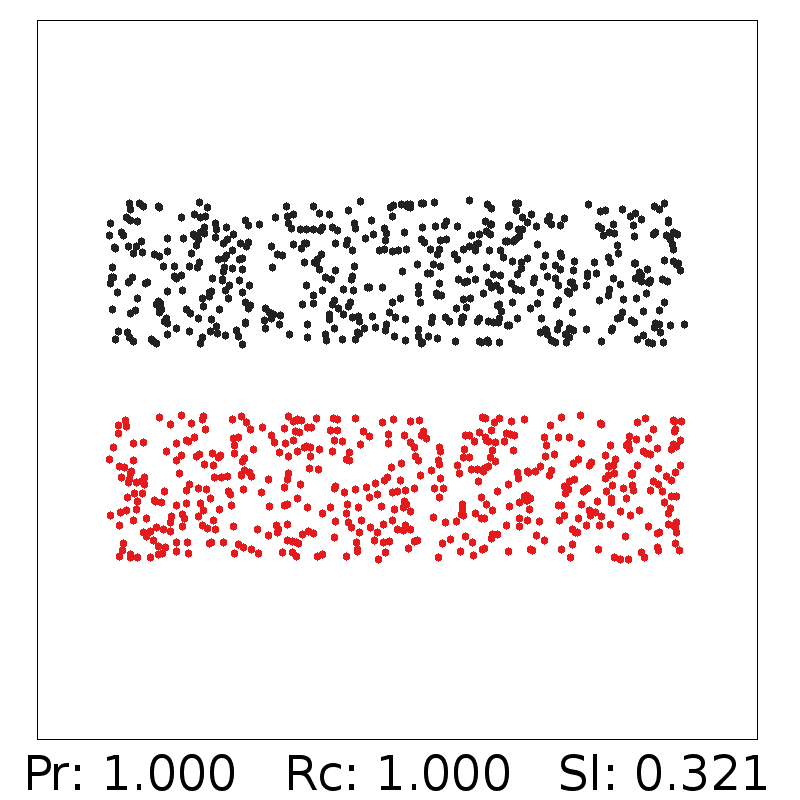
\includegraphics[scale=0.2]{{{../results-usable-clus/oblong.truth}}}
	\caption{Ground truth}
	\label{fig:expected-oblong}
	\end{subfigure}%	
	\begin{subfigure}[b]{0.3\textwidth}
	\centering
	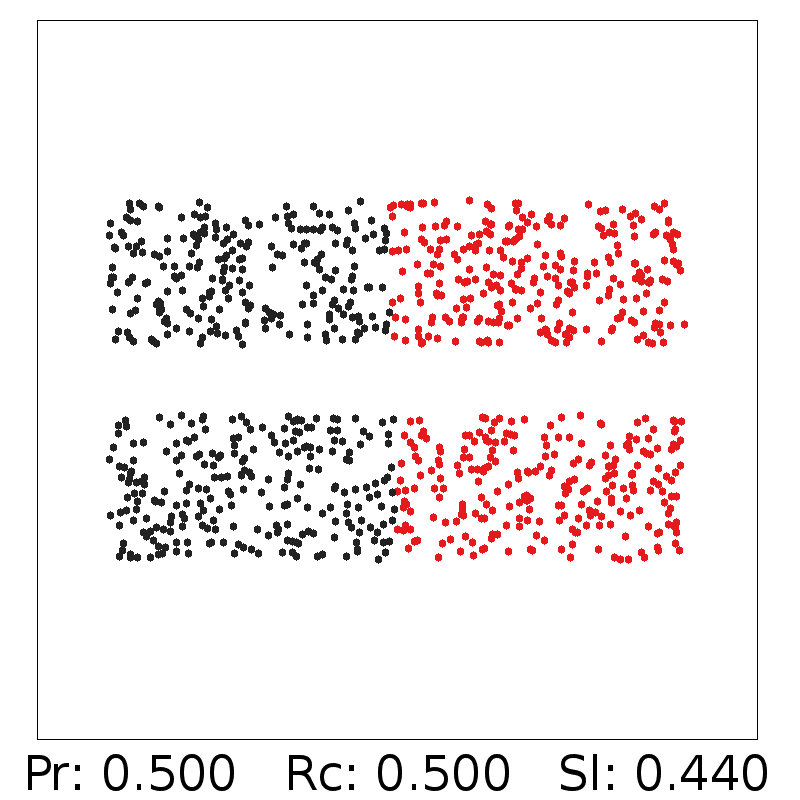
\includegraphics[scale=0.2]{{{../results-usable-clus/oblong.kmeans}}}
	\caption{$k$-means}
	\label{fig:kmeans-oblong}
	\end{subfigure}%
	\begin{subfigure}[b]{0.3\textwidth}
	\centering
	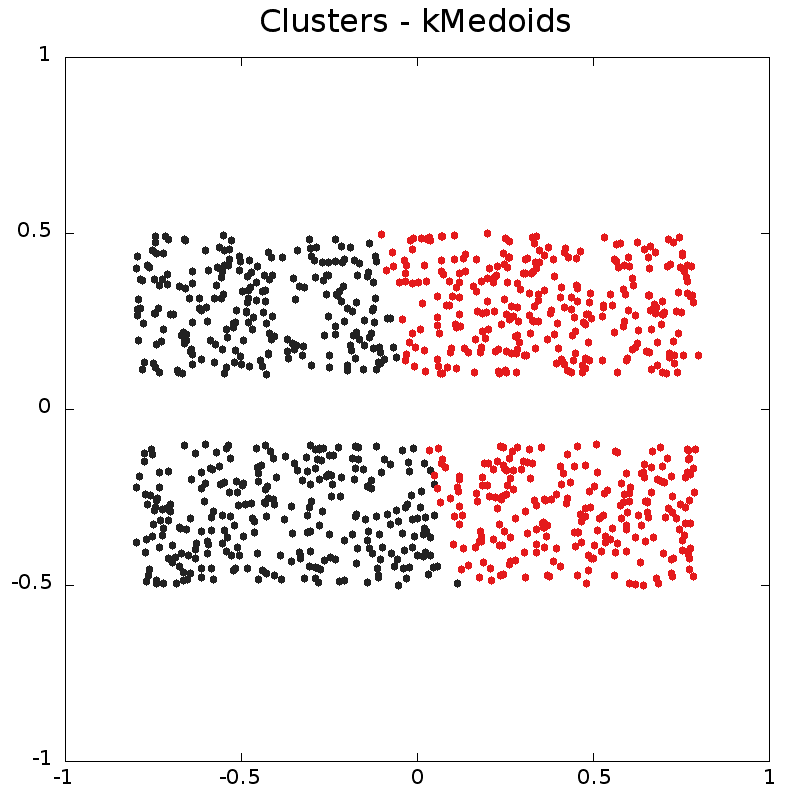
\includegraphics[scale=0.2]{{{../results-usable-clus/oblong.kmedoids}}}
	\caption{PAM}
	\label{fig:kmedoids-oblong}
	\end{subfigure}	
	\begin{subfigure}[b]{0.3\textwidth}
	\centering
	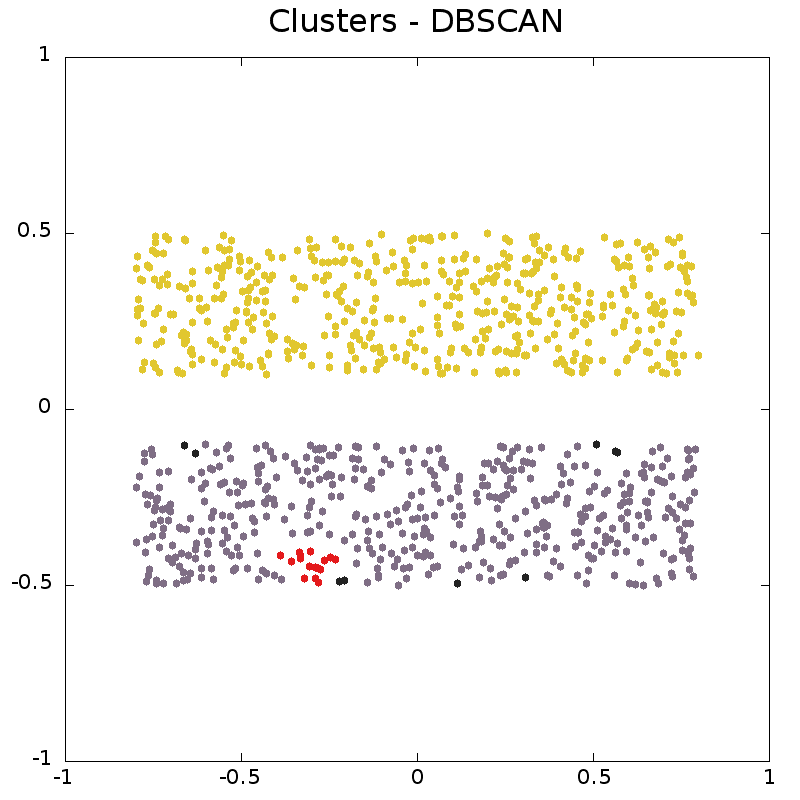
\includegraphics[scale=0.2]{{{../results-usable-clus/oblong.dbscan}}}
	\caption{DBSCAN}
	\label{fig:dbscan-oblong}
	\end{subfigure}%
	\begin{subfigure}[b]{0.3\textwidth}
	\centering
	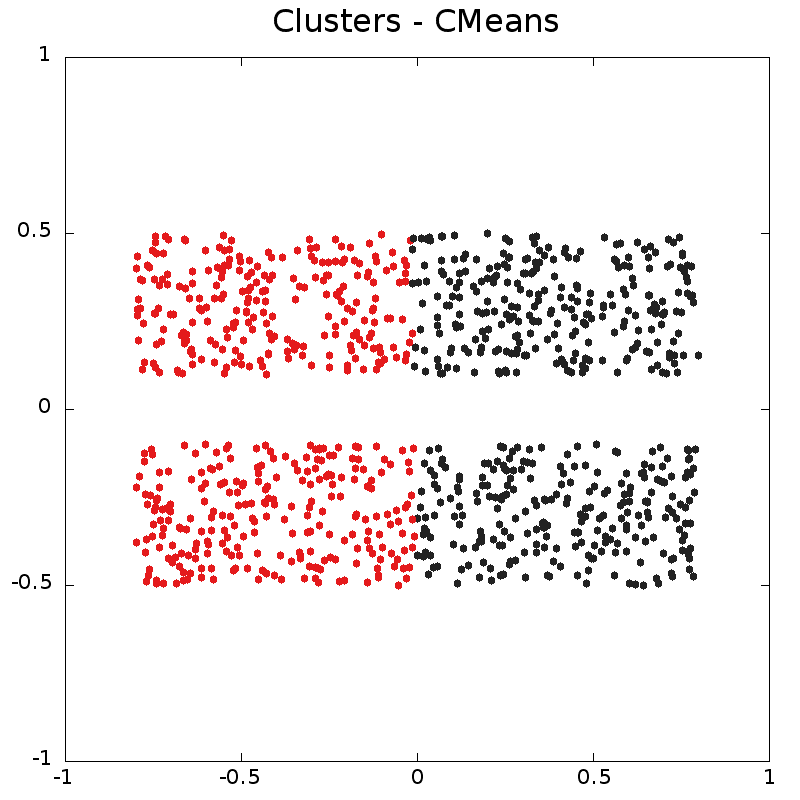
\includegraphics[scale=0.2]{{{../results-usable-clus/oblong.cmeans}}}
	\caption{EM}
	\label{fig:cmeans-oblong}
	\end{subfigure}
\caption{Clustering results on two oblong clusters.}
\label{fig:oblong}
\end{figure}

\begin{figure}[h]
	\centering
	\begin{subfigure}[b]{\textwidth}
	\centering
	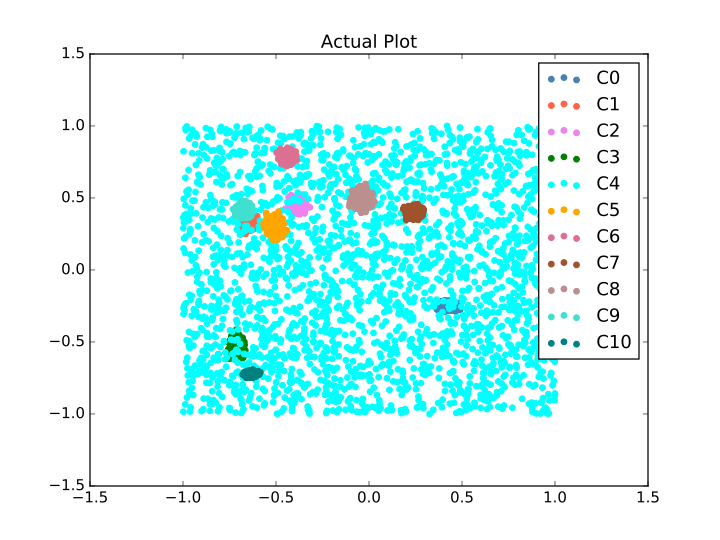
\includegraphics[scale=0.3]{{{../neeraj-plots/Actual}}}
	\caption{Original data}
	\label{fig:expected-clusters}
	\end{subfigure}
	
	\begin{subfigure}[b]{0.5\textwidth}
	\centering
	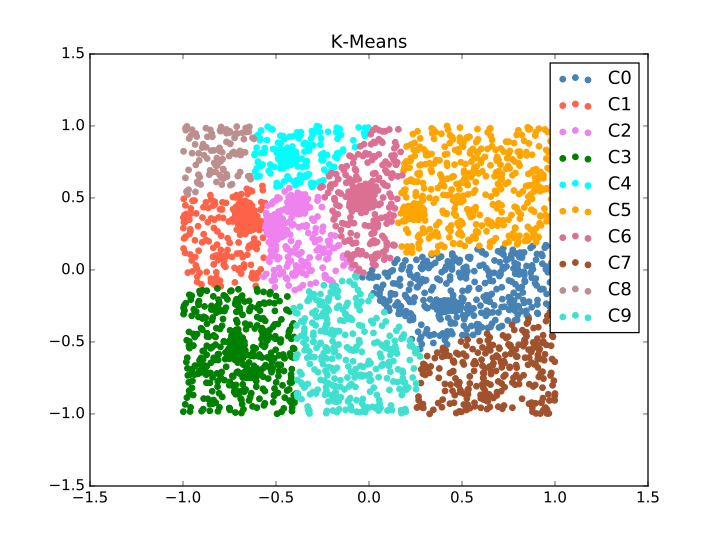
\includegraphics[scale=0.3]{{{../neeraj-plots/Kmeans}}}
	\caption{$k$-means.}
	\label{fig:kmeans-clusters}
	\end{subfigure}%
	\begin{subfigure}[b]{0.5\textwidth}
	\centering
	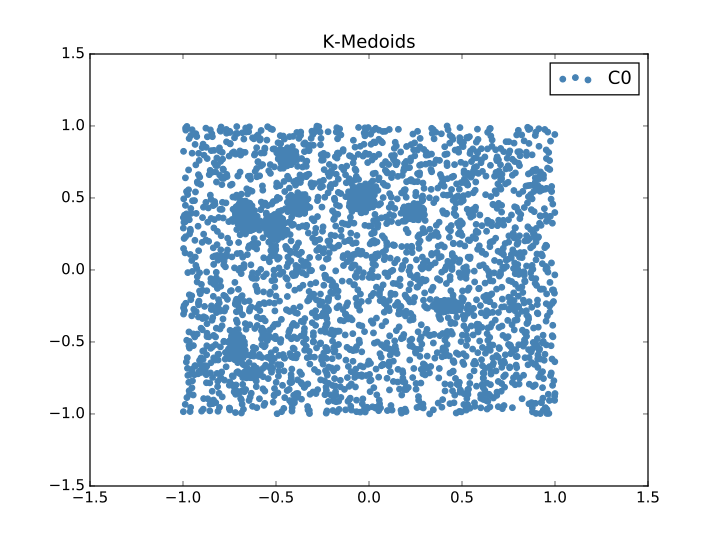
\includegraphics[scale=0.3]{{{../neeraj-plots/Kmedoids}}}
	\caption{PAM}
	\label{fig:kmedoids-clusters}
	\end{subfigure}
	
	\begin{subfigure}[b]{0.5\textwidth}
	\centering
	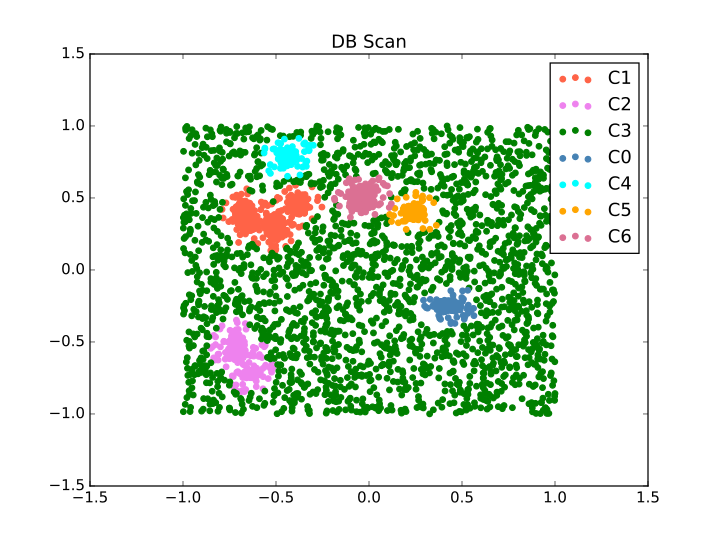
\includegraphics[scale=0.3]{{{../neeraj-plots/Dbscan}}}
	\caption{DBSCAN}
	\label{fig:dbscan-clusters}
	\end{subfigure}%
	\begin{subfigure}[b]{0.5\textwidth}
	\centering
	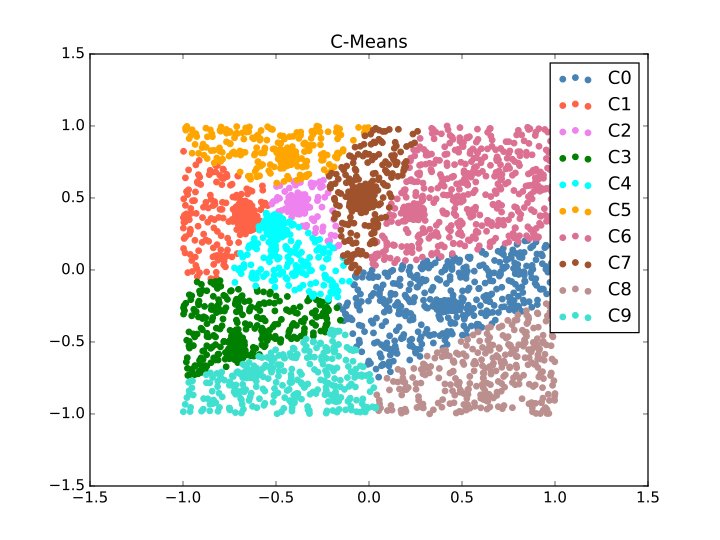
\includegraphics[scale=0.3]{{{../neeraj-plots/Cmeans}}}
	\caption{EM}
	\label{fig:em-clusters}
	\end{subfigure}
	
	\caption{Clustering results from an earlier version of the data generator.}
	\label{fig:cluster-assignments}
\end{figure}
\end{document}